\documentclass[border=2pt,multi=tikzpicture]{standalone}
\usepackage{tikz}
\usetikzlibrary{positioning, arrows.meta, calc, fit}
\definecolor{acc}{RGB}{28,60,102}
\newcommand{\stepnum}[1]{\tikz[baseline=-0.62ex]{\node[circle,fill=acc,text=white,
  inner sep=0.25mm, minimum size=3.1mm, font=\tiny\bfseries]{#1};}}
\tikzset{
  arr/.style={-{Latex[length=1.8mm,width=1.5mm]}, semithick, draw=black!80},
  barr/.style={-{Latex[length=1.8mm,width=1.5mm]}, semithick, draw=black!80, densely dashed},
  bbarr/.style={{Latex[length=1.8mm,width=1.5mm]}-{Latex[length=1.8mm,width=1.5mm]},
    semithick, draw=black!80, densely dashed},
  darr/.style={{Latex[length=1.5mm,width=1.3mm]}-{Latex[length=1.5mm,width=1.3mm]},
    semithick, draw=black!80},
  blk/.style={draw=black!45, rounded corners=1.6pt, align=center, inner sep=2.4pt, fill=white},
  lab/.style={font=\tiny, align=center, inner sep=1.2pt, fill=white},
  panel/.style={fill=black!4, draw=black!25, rounded corners=3.5pt},
  zlab/.style={font=\tiny\bfseries\scshape, text=acc, fill=white, inner sep=1.6pt},
  zone/.style={draw=black!50, densely dashed, rounded corners=3pt}
}
\begin{document}
% ================== FIG 1: SYSTEM ARCHITECTURE (strict grid) ==================
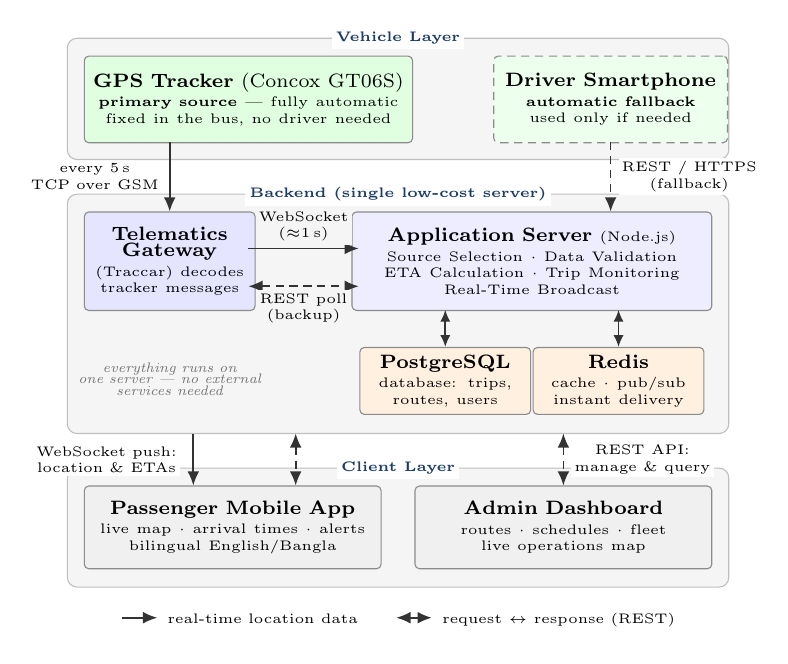
\begin{tikzpicture}[font=\scriptsize, x=1mm, y=1mm]
% ---------- layer panels (drawn first, boxes on top) ----------
\draw[panel] (-42, 2.2) rectangle ( 42,-13.2);
\draw[panel] (-42,-17.6) rectangle ( 42,-48.0);
\draw[panel] (-42,-52.4) rectangle ( 42,-67.5);
\node[zlab] at (0, 2.2)  {Vehicle Layer};
\node[zlab] at (0,-17.6) {Backend (single low-cost server)};
\node[zlab] at (0,-52.4) {Client Layer};
% ---------- vehicle layer ----------
\node[blk, fill=green!12, text width=40mm, minimum height=11mm, anchor=north] (gt) at (-19,0)
  {\textbf{GPS Tracker} (Concox GT06S)\\[-1pt]
   {\tiny \textbf{primary source} --- fully automatic}\\[-2pt]
   {\tiny fixed in the bus, no driver needed}};
\node[blk, fill=green!7, densely dashed, text width=28mm, minimum height=11mm, anchor=north]
  (ph) at (27,0)
  {\textbf{Driver Smartphone}\\[-1pt]
   {\tiny \textbf{automatic fallback}}\\[-2pt]
   {\tiny used only if needed}};
% ---------- backend layer ----------
\node[blk, fill=blue!10, text width=20mm, minimum height=12.5mm, anchor=north] (trac) at (-29,-19.8)
  {\textbf{Telematics}\\[-2pt]\textbf{Gateway}\\[-1pt]
   {\tiny (Traccar) decodes}\\[-2pt]{\tiny tracker messages}};
\node[blk, fill=blue!7, text width=44mm, minimum height=12.5mm, anchor=north] (app) at (17,-19.8)
  {\textbf{Application Server} {\tiny(Node.js)}\\[-1pt]
   {\tiny Source Selection $\cdot$ Data Validation}\\[-2pt]
   {\tiny ETA Calculation $\cdot$ Trip Monitoring}\\[-2pt]
   {\tiny Real-Time Broadcast}};
\node[blk, fill=orange!12, text width=20mm, minimum height=8.5mm, anchor=north] (pg) at (6,-37.0)
  {\textbf{PostgreSQL}\\[-1pt]{\tiny database: trips,}\\[-2pt]{\tiny routes, users}};
\node[blk, fill=orange!12, text width=20mm, minimum height=8.5mm, anchor=north] (rd) at (28,-37.0)
  {\textbf{Redis}\\[-1pt]{\tiny cache $\cdot$ pub/sub}\\[-2pt]{\tiny instant delivery}};
\node[font=\tiny\itshape, text=black!55, align=center] at (-29,-41.1)
  {everything runs on\\[-2pt]one server --- no external\\[-2pt]services needed};
% ---------- client layer ----------
\node[blk, fill=black!6, text width=36mm, minimum height=10.5mm, anchor=north] (pass) at (-21,-54.6)
  {\textbf{Passenger Mobile App}\\[-1pt]
   {\tiny live map $\cdot$ arrival times $\cdot$ alerts}\\[-2pt]
   {\tiny bilingual English/Bangla}};
\node[blk, fill=black!6, text width=36mm, minimum height=10.5mm, anchor=north] (adm) at (21,-54.6)
  {\textbf{Admin Dashboard}\\[-1pt]
   {\tiny routes $\cdot$ schedules $\cdot$ fleet}\\[-2pt]
   {\tiny live operations map}};
% ---------- connections (all verticals aligned to fixed x) ----------
\draw[arr]  (-29,-11) -- (-29,-19.8)
  node[lab, midway, anchor=east, xshift=-0.9mm] {every 5\,s\\TCP over GSM};
\draw[barr] ( 27,-11) -- ( 27,-19.8)
  node[lab, midway, anchor=west, xshift=0.9mm] {REST / HTTPS\\(fallback)};
\draw[arr]  (-19,-24.5) -- (-5,-24.5)
  node[lab, midway, anchor=south, yshift=0.4mm, fill=black!4] {WebSocket\\($\approx$1\,s)};
\draw[bbarr] (-19,-29.3) -- (-5,-29.3)
  node[lab, midway, anchor=north, yshift=-0.4mm, fill=black!4] {REST poll\\(backup)};
\draw[darr] ( 6,-32.3) -- ( 6,-37.0);
\draw[darr] (28,-32.3) -- (28,-37.0);
\draw[arr]  (-26,-48.0) -- (-26,-54.6)
  node[lab, midway, anchor=east, xshift=-1.6mm] {WebSocket push:\\location \& ETAs};
\draw[bbarr] (-13,-48.0) -- (-13,-54.6);
\draw[bbarr] ( 21,-48.0) -- ( 21,-54.6)
  node[lab, midway, anchor=west, xshift=0.9mm] {REST API:\\manage \& query};
% ---------- legend ----------
\node[anchor=north, font=\tiny] at (0,-69.4)
  {\tikz{\draw[arr] (0,0) -- (4.5mm,0);}\, real-time location data\qquad
   \tikz{\draw[bbarr] (0,0) -- (4.5mm,0);}\, request $\leftrightarrow$ response (REST)};
\end{tikzpicture}
% ================== FIG 2: REAL-TIME DATA FLOW (uniform grid) ==================
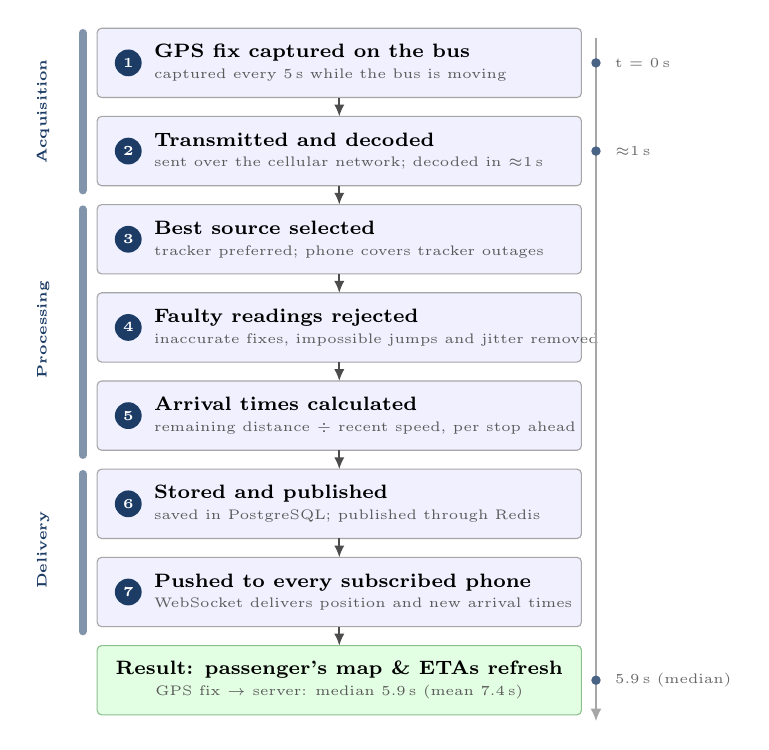
\begin{tikzpicture}[font=\scriptsize, x=1mm, y=1mm,
  stp/.style={draw=black!35, rounded corners=1.6pt, fill=blue!6, align=left,
              text width=58mm, minimum height=8.8mm, inner sep=2.2pt, anchor=north},
  sarr/.style={-{Latex[length=1.5mm,width=1.3mm]}, semithick, draw=black!70},
  phl/.style={font=\tiny\bfseries\scshape, text=acc, rotate=90, anchor=south}]
% ---- steps on a uniform grid: height 8.8, gap 2.4 ----
\foreach \y/\n/\t/\d in {
  0/1/{GPS fix captured on the bus}/{captured every 5\,s while the bus is moving},
  -11.2/2/{Transmitted and decoded}/{sent over the cellular network; decoded in $\approx$1\,s},
  -22.4/3/{Best source selected}/{tracker preferred; phone covers tracker outages},
  -33.6/4/{Faulty readings rejected}/{inaccurate fixes, impossible jumps and jitter removed},
  -44.8/5/{Arrival times calculated}/{remaining distance $\div$ recent speed, per stop ahead},
  -56.0/6/{Stored and published}/{saved in PostgreSQL; published through Redis},
  -67.2/7/{Pushed to every subscribed phone}/{WebSocket delivers position and new arrival times}}{
  \draw[draw=black!35, rounded corners=1.6pt, fill=blue!6]
    (-30.75,\y) rectangle (30.75,\y-8.8);
  \node[circle, fill=acc, text=white, inner sep=0.25mm, minimum size=3.4mm,
        font=\tiny\bfseries] at (-26.8,\y-4.4) {\n};
  \node[anchor=west, align=left, inner sep=0pt] at (-23.6,\y-4.4)
    {\textbf{\t}\\[-0.5pt]{\tiny\color{black!65} \d}};
}
\draw[draw=green!45!black!45, rounded corners=1.6pt, fill=green!11]
  (-30.75,-78.4) rectangle (30.75,-87.2);
\node[align=center] at (0,-82.8)
  {\textbf{Result: passenger's map \& ETAs refresh}\\[-0.5pt]
   {\tiny\color{black!65} GPS fix $\rightarrow$ server: median 5.9\,s (mean 7.4\,s)}};
% ---- identical arrows (2.4 mm each) ----
\foreach \y in {-8.8,-20.0,-31.2,-42.4,-53.6,-64.8,-76.0}{
  \draw[sarr] (0,\y) -- (0,\y-2.4);}
% ---- phase bars (left, uniform) ----
\foreach \ya/\yb/\nm in {0/-20.0/Acquisition, -22.4/-53.6/Processing, -56.0/-76.0/Delivery}{
  \draw[acc!55, line width=1mm, line cap=round] (-32.6,\ya-0.6) -- (-32.6,\yb-0.6);}
\node[phl] at (-35.6,-10.6) {Acquisition};
\node[phl] at (-35.6,-38.3) {Processing};
\node[phl] at (-35.6,-66.3) {Delivery};
% ---- timeline (right) ----
\draw[black!35, line width=0.6pt, -{Latex[length=1.6mm,width=1.4mm]}]
  (32.6,-1.2) -- (32.6,-88.0);
\foreach \y/\t in {-4.4/{t $=$ 0\,s}, -15.6/{$\approx$1\,s}, -82.8/{5.9\,s (median)}}{
  \fill[acc!80] (32.6,\y) circle (0.6mm);
  \node[font=\tiny, anchor=west, text=black!60] at (33.8,\y) {\t};}
\end{tikzpicture}
\end{document}
